% TODO: FIX LATEX ERRORS
\chapter{Technische Grundlagen}
\section{\acf{OLAP}}
Viele Unternehmen verwenden heute große Mengen an Geschäftsdaten für eine strategische Planung.
Durch eine Analyse der Daten lassen sich Handlungsempfehlungen ableiten.
Typische Analysen umfassen die Berechnung des Umsatzes einer Filiale innerhalb des letzten Jahres sowie der Vergleich zu vorherigen Jahren oder die Analyse der Verkäufe von einzelnen Produkten in einem bestimmten Quartal.
Diese Analysen erfordern eine umfassende Datenmenge, einschließlich historischer Daten.
Klassische Datenbanksysteme für Transaktionen, etwa in einem Onlineshop, auch \acf{OLTP} genannt, sind für viele Schreib- und Lesezugriffe optimiert, nutzen meist wenig komplexe Abfragen (Queries) und enthalten häufig keine historischen Daten.
Datenbanken für analytische Zwecke sollten hingegen stark auf die Leseoperationen optimiert sein und müssen komplexere Queries in angemessener Zeit durchführen können.
Bei diesem Einsatzgebiet von Datenbanken spricht man vom \acf{OLAP}~\cite[S.~97f]{kleppmann_datenintensive_2019}.

\ac{OLAP} und \ac{OLTP} profitieren von verschiedenen Optimierungen der Datenstrukturen in einer Datenbank.
Bei Nutzung einer gemeinsamen Datenbank für beide Verfahren würden die \ac{OLAP}-Abfragen außerdem die \ac{OLTP}-Transaktionen verlangsamen oder blockieren.
Um das zu verhindern, nutzt man für \ac{OLAP} eigene Datenbanksysteme und speichert die Daten in sogenannten Data Warhouses.

\subsection{\acfp{DW}}
\acp{DW} wurden entwickelt, um Daten zu speichern, die für strategische Entscheidungen im Geschäftsumfeld nützlich sein können.
Dazu werden Daten aus Geschäftsprozessen wie etwa Verkäufen extrahiert, für die weitere Verwendung transformiert und in bestimmten Datenbanken gespeichert.
Klassische  operative oder transaktionale Datenbankansätze, die auf den täglichen Gebrauch durch viele Nutzende optimiert sind, eignen sich nicht für ein \ac{DW} im \ac{OLAP}-Umfeld, da hier üblicherweise keine historischen Daten gespeichert werden.
Des Weiteren enthalten diese detaillierte Daten, was das Ausführen von komplexen Abfragen erschwert bzw. verlangsamt.
% Hier ähnliche Inhalte wie im Kapitel weiter oben
Um aber Entscheidungen aus den Daten ableiten zu können, sind sowohl historische Daten als auch komplexe Abfragen notwendig.
Um diese Probleme zu lösen, enthält ein \ac{DW} im \ac{OLAP} Umfeld historische Daten und bietet ein optimiertes Datenmodell für komplexere Abfragen.
In der ursprünglichen Definition nach Inmon werden \acp{DW} als Sammlung von subjektorientierten, integrierten, nicht flüchtigen und zeitvariablen Daten beschrieben. % TODO: Hier wäre Originalquelle ganz praktisch
Subjektorientiert bedeutet, dass sich die Daten auf bestimmte Aspekte der geforderten Analyse beziehen, also z.~B. Daten über Produktionsmengen und Verkäufen bei Produktionsunternehmen.
Mit integrierten Daten ist gemeint, dass Daten aus verschiedenen Umgebungen in dem \ac{DW} integriert sind.
Nicht flüchtig bedeutet, dass die Daten über lange Zeiträume hinweg gespeichert bleiben und somit weder gelöscht noch modifiziert werden.
Zur Analyse ist es wichtig, Daten im zeitlichen Verlauf miteinander zu vergleichen, etwa um herauszufinden, wie sich die Verkäufe im letzten Quartal entwickelt haben.
Zeitvariabel beschriebt daher, dass Daten aus verschiedenen Zeitpunkten gespeichert werden~\cite[S.~3f]{vaisman_data_2022}.

\subsection{Datenstruktur in Data Warehouses im \ac{OLAP} Umfeld}
Die Mehrheit der am häufigsten verwendeten Datenbanken nutzt ein relationales Datenbankmodell~\cite{db-engines_most_2023}. 
In einem solchen Modell können die Daten in verschiedenen Schemata aufgebaut sein.

\subsubsection{Normalisierung}
Eine gängige Praxis bei relationalen Datenbanken ist die Normalisierung.
Ziel der Normalisierung ist das Verhindern von redundanten Daten.
Enthalten mehrere Tabellen die gleichen Daten, so müssen diese Daten an mehreren Stellen bei Änderungen angepasst werden.
Um diesen Umstand zu verhindern, werden die Daten daher nur in einer Tabelle gespeichert und dann per Fremdschlüssel in den anderen Tabellen eingebunden~\cite[S.~24f]{vaisman_data_2022}.
Diese Fremdschlüssel benötigen in den meisten Fällen außerdem weniger Speicherplatz als die eigentlichen Daten, was einen weiteren Vorteil bietet.
Ein Nachteil der Normalisierung ist jedoch, dass Abfragen komplizierter werden und länger in der Ausführung benötigen, da die Daten aus verschiedenen Tabellen kombiniert werden müssen.

\subsubsection{Sternschema und Schneeflockenschema}
In \acp{DW}, die für große Datenmengen und komplexe Abfragen gedacht sind, bildet das Normalisieren durch die erschwerten Abfragen einen Nachteil.
Um Daten für Abfragen effizient zu speichern, werden diese nicht so weit wie möglich normalisiert, sondern anhand ihrer Inhalte verteilt. 
Durch Verständnis der Daten können diese in eine sogenannte Faktentabelle und viele Dimensionstabellen aufgeteilt werden.

In der Faktentabelle befinden sich die zentralen Metriken, die zur Analyse benötigt werden, etwa die Anzahl der Verkäufe eines Produktes.
Die Dimensionstabellen enthalten Daten, mit denen die Daten der Faktentabelle unter verschiedenen Umständen betrachtet werden können, etwa eine Dimensionstabelle mit Zeitpunkten oder Orten.
Diese Dimensionstabellen sind mit der Faktentabelle über Fremdschlüssel verbunden.

In einem Diagramm werden die Dimensionstabellen um die Faktentabelle angeordnet, wodurch das Diagramm einem Stern ähnelt, bei dem die Faktentabelle das Zentrum, und die Dimensionen die Strahlen bilden.
Deshalb spricht man auch von einem Sternschema.
Werden die Faktentabellen zusätzlich noch unterteilt, die Daten also noch normalisiert, spricht man von einem Schneeflockenschema.
Wie oben beschrieben eignen sich nicht normalisierte Daten jedoch besser für analytische Abfragen, weshalb das Sternschema oft bevorzugt wird.

Die Faktentabelle enthält den Großteil der Daten.
Jedes Ereignis wird in einer eigenen Zeile gespeichert, um somit so detailreich wie möglich analysieren zu können.
Des Weiteren kann die Faktentabelle sehr viele Spalten mit Details zu den Ereignissen enthalten.
Dimensionstabellen sind dahingegen wesentlich kleiner\cite[S.~101-103]{kleppmann_datenintensive_2019}.

Bei Abfragen können nun verschiedene Dimensionen kombiniert werden, um Daten aus der Faktentabelle abzufragen.
So können z.~B. die Verkäufe aus einem bestimmten Jahr in einer bestimmten Filiale aus der Faktentabelle abgefragt werden.
Die Dimensionstabellen können außerdem sogenannte Hierarchien enthalten, die verschiedene Genauigkeiten der Dimension definieren.
So kann ein Zeitpunkt in der Tabelle Werte für Uhrzeit, Tag, Monat, Quartal oder Jahr enthalten.
Ein Ort kann etwa aus dem Ortsnamen, dem Bundesland, dem Land, dem Kontinent bestehen.
So lassen sich genaue Abfragen zu Verkäufen einer bestimmten Filiale oder etwa allen Filialen in Europa abfragen~\cite[S.~5]{vaisman_data_2022}.

\begin{comment}
\subsection{Der OLAP-Cube}
%TODO: OLAP CUBE Voraggregation bei OLAP -> Kleppmann Seite 109 Kapitel 3


% Tabelle überdenken
\begin{table}[htbp] 
    \centering
    \footnotesize
    \begin{tabular}{ccccc}
        \toprule  
        Id & Umsatz & Stückzahl & Zeit & Ort \\
        \midrule
        1 & 100,00 € & 50 & 1 & 1 \\
        2 & 200,00 € & 100 & 2 & 2 \\
        3 & 150,00 € & 75 & 3 & 3 \\
        \bottomrule
    \end{tabular}
    \caption{Faktentabelle mit Umsatz, Stückzahl, Zeit und Ort}
    \label{tab:faktentabelle}
\end{table}

\begin{table}[htbp] 
    \centering
    \footnotesize
    \begin{tabular}{cccccc}
        \toprule  
        Id & Ortsname & Postleitzahl & Landkreis & Bundesland & Land \\
        \midrule
        1 & Furtwangen & 78120 & Schwarzwald-Baar-Kreis & Baden-Württemberg & Deutschland \\
        2 & Schömberg & 75328 & Landkreis Calw & Baden-Württemberg & Deutschland \\
        3 & Pforzheim & 75173 & Enzkreis & Baden-Württemberg & Deutschland \\
        \bottomrule
    \end{tabular}
    \caption{Ortstabelle mit Ortsname, Postleitzahl, Landkreis, Bundesland und Land}
    \label{tab:ortstabelle}
\end{table}

\begin{table}[htbp] 
    \centering
    \footnotesize
    \begin{tabular}{cccccc}
        \toprule  
        Id & Timestamp & Datum & Monat & Quartal & Jahr \\
        \midrule
        1 & 02.12.1998 12:00 & 02.12.1998 & Dezember & 4 & 1998 \\
        2 & 28.12.2007 12:00 & 02.01.2007 & Januar & 1 & 2007 \\
        3 & 03.01.2023 16:00 & 03.01.2023 & Januar & 1 & 2023 \\
        \bottomrule
    \end{tabular}
    \caption{Zeittabelle mit Timestamp, Datum, Monat, Quartal und Jahr}
    \label{tab:zeittabelle}
\end{table}


% Eventuell Kapitel über Query Languages schreiben
\subsection{Die \acs{SQL}-Sprache} % Titel verbessern
% Code Listing ist auf englisch, zu deutsch ändern
\begin{lstlisting}[
    language=SQL,
    caption=SQL Befehle zum Anlegen der Tabellen,
    label=code:sql-creation-of-tables
]
CREATE TABLE Ortstabelle (
    Id INT PRIMARY KEY,
    Ortsname VARCHAR(255),
    Postleitzahl CHAR(5),
    Landkreis VARCHAR(255),
    Bundesland VARCHAR(255),
    Land VARCHAR(255)
);

CREATE TABLE Zeittabelle (
    Id INT PRIMARY KEY,
    Timestamp TIMESTAMP,
    Datum DATE,
    Monat VARCHAR(255),
    Quartal SMALLINT,
    Jahr SMALLINT
);

CREATE TABLE Faktentabelle (
    Id INT PRIMARY KEY,
    Umsatz VARCHAR(255),
    Stueckzahl INT,
    Zeit INT,
    Ort INT,
    FOREIGN KEY (Zeit) REFERENCES Zeittabelle(Id),
    FOREIGN KEY (Ort) REFERENCES Ortstabelle(Id)
);

\end{lstlisting}

In \cref{code:sql-creation-of-tables} werden \acs{SQL}-Befehle zum Erstellen der Beispieltabellen dargestellt.
In den Befehlen werden die einzelnen Spalten der Tabelle mit ihren Datentypen angelegt.
Verschiedene \acs{SQL}-Erweiterungen unterstützen verschiedene Datentypen, mit denen Daten teilweise effizienter gespeichert werden können.
So bietet die \acs{SQL}-Erweiterung Transact-\acs{SQL} von Microsoft noch den Datentyp TINYINT der einen Wert von 0 bis 255 annehmen kann~\cite{ray_et_al_int_2023} und für die Spalte Quartal gut genutzt werden könnte.
PostgreSQL bietet hingegen keinen solchen Datentypen~\cite{the_postgresql_global_development_group_81_2023} und da im Verlauf dieser Arbeit mit PostgreSQL gearbeitet wurde, wird auch in diesem Beispiel kein TINYINT verwendet.

\end{comment}



\subsection{\acf{OLAP}}

\subsection{Key Value Stores in \acs{OLAP}}

\section{Datenbank-Benchmarks}
Datenbank-Benchmarks geben einen Überblick über die Leistung von verschiedenen Datenbanksysteme und die Hardware, auf der diese laufen.
%Datenbank-Benchmark oder Datenbankbenchmark ?
Die Non-Profit-Organisation \acf{TPC} hat verschiedene Datenbank-Benchmarks entwickelt, die bei der Wahl des Datenbanksystems oder der Hardware helfen können~\cite[s. 619]{barata_overview_2015}.

\subsection{\acf{TPC-H}}
Der \acf{TPC-H} wurde zum Testen von analytischen Datenbanken entwickelt.
Die Daten und Abfragen des Benchmarks sind auf eine Datenbank ausgelegt, mit der ein Anbieter seine Geschäftsdaten analysieren kann~\cite[S.~624-626]{barata_overview_2015}

\subsection{\acf{SSB}}
Der \acf{SSB} ist eine abgewandelte Form des \ac{TPC-H}.

\subsubsection{Schema des \ac{SSB}}
Er verwendet die gleichen Daten, nutzt dafür jedoch ein Sternschema statt eines normalisierten Schemas.
Um die Daten an ein Sternschema anzupassen, wurden die normalisierte Struktur des \ac{TPC-H} denormalisiert.
Somit wurden einige Tabellen zusammengelegt.
Außerdem wurden einige, für OLAP unwichtige, Daten entfernt.
Im Paper~\cite{oneil_star_2009} zum \ac{SSB} werden die Änderungen im Detail beschrieben.
% Hier habe ich mich bewusst dazu entschieden, nicht darauf einzugehen, welche Tabellen aus TPC-H wie verändert wurden, da TPC-H irrelevant für diese Arbeit ist.
Nach den Anpassungen sind die Daten in einer Faktentabelle namens LINEORDER sowie den Dimensionstabellen CUSTOMER, PART, SUPPLIER und DATE organisiert (siehe Abbildung~\ref{pic:ssb-schema}).
Die Felder innerhalb der Tabellen beginnen mit einem Präfix, bestehend aus dem Anfangsbuchstaben der Tabelle und einem Unterstrich, also etwa d\_year in der DATE-Tabelle.

\begin{figure}[ht]  % figure position
    \centering      % center the image
    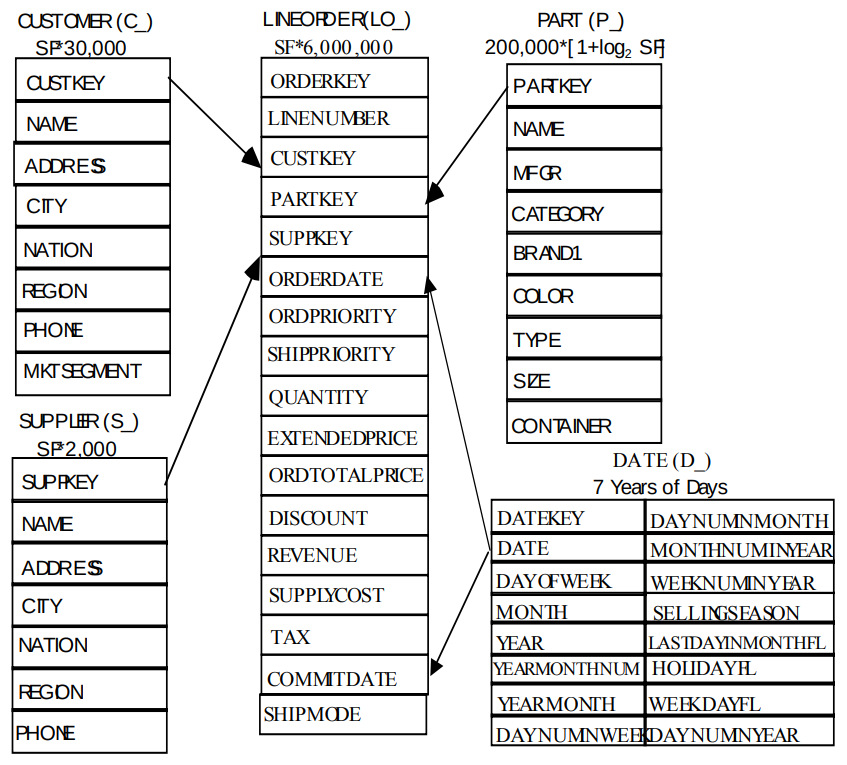
\includegraphics[width=1\textwidth]{pictures/ssb/ssb-schema.png}
    \caption{Schema des \ac{SSB}~\cite{oneil_star_2009}}      % caption the image
    \label{pic:ssb-schema}    % label the image for internal referencing
\end{figure}


\subsubsection{Queries des \ac{SSB}}
Die Queries des \ac{SSB} unterscheiden sich von denen des \ac{TPC-H}.
Der \ac{SSB} nutzt nur Queries, die genau eine SELECT-Anweisung auf der Faktentabelle LINEORDER nutzen und somit keine self-joins nutzen. %self-joins bissl weirder Ausdruck
Die LINEORDER Tabelle wird dann mit einer oder mehreren Dimensionstabellen gejoint und die Ergebnisse somit gefiltert. 
%TODO: Alle SSB SQL-Queries in den Anhang packen

Die Queries des \ac{SSB} sind in vier Kategorien aufgeteilt (query flights): % query flights bissl weird

%TODO: \usepackage{underscore}

\paragraph{Q1}
%ausbauen
Queries in Q1 schränken die Daten über nur eine Dimension, \textbf{DATE}, ein.
Die Faktentabelle \emph{LINEORDER} wird mit der Dimensionstabelle\emph{DATE} gejoint und die Daten anhand einer Zeitspanne aus der DATE-Tabelle und den Bereichen der Felder \emph{lo\_discount} und \emph{lo\_quantity} aus der LINEORDER-Tabelle gefiltert.
Anschließend wird der Umsatz als Summe der Produkte der Felder \emph{lo\_extendedprice} und \emph{lo\_discount} berechnet und als \emph{revenue} zurückgegeben \cite{oneil_star_2009}.


\begin{lstlisting}[
    language=SQL,
    caption=SQL Query-Struktur für Q1 des \ac{SSB},
    label=code:ssb-q1-structur-example
]
SELECT 
    SUM(lo_extendedprice * lo_discount) AS revenue
FROM 
    lineorder, date
WHERE 
    lo_orderdate = d_datekey
    AND d_year = [YEAR]
    -- Specific values below
    AND lo_discount BETWEEN [DISCOUNT] - 1 AND [DISCOUNT] + 1
    AND lo_quantity < [QUANTITY];
\end{lstlisting}

\paragraph{Q2}
In Q2 schränken die Queries die Daten über zwei Dimensionen ein: \textbf{PART} und \textbf{SUPPLIER}.
Anschließend wird wie in Q1 der Umsatz gebildet, wobei die Ergebnisse hier noch nach \emph{d\_year} und \emph{p\_brand1} gruppiert und sortiert werden.  
In Q2 werden insgesamt vier Tabellen (\emph{LINEORDER}, \emph{PART}, \emph{SUPPLIER}, \emph{DATE}) gejoint.
\begin{lstlisting}[
    language=SQL,
    caption=SQL Query-Struktur für Q2 des \ac{SSB},
    label=code:ssb-q2-structur-example
]
SELECT 
    SUM(lo_revenue) AS total_revenue, d_year, p_brand1
FROM 
    lineorder, date, part, supplier
WHERE 
    lo_orderdate = d_datekey
    AND lo_partkey = p_partkey
    AND lo_suppkey = s_suppkey
    AND p_category = 'MFGR#12'
    AND s_region = 'AMERICA'
GROUP BY 
    d_year, p_brand1
ORDER BY 
    d_year, p_brand1;

\end{lstlisting}

\paragraph{Q3}
In Q3 schränken die Queries die Daten über drei Dimensionen ein: \textbf{DATE}, \textbf{SUPPLIER} und \textbf{CUSTOMER}.
Wie in Q1 und Q2 werden auch hier die Umsätze gebildet.
Anschließend werden sie nach \emph{c\_nation}, \emph{s\_region} und \emph{d\_year} gruppiert und nach \emph{d\_year} sortiert.
Es werden insgesamt vier Tabellen (\emph{LINEORDER}, \emph{DATE}, \emph{SUPPLIER} und \emph{CUSTOMER}) gejoint.
\begin{lstlisting}[
    language=SQL,
    caption=SQL Query-Struktur für Q3 des \ac{SSB},
    label=code:ssb-q3-structur-example
]
SELECT 
    c_nation, s_nation, d_year, SUM(lo_revenue) AS revenue
FROM 
    customer, lineorder, supplier, date
WHERE 
    lo_custkey = c_custkey
    AND lo_suppkey = s_suppkey
    AND lo_orderdate = d_datekey
    AND c_region = 'ASIA'
    AND s_region = 'ASIA'
    AND d_year >= 1992
    AND d_year <= 1997
GROUP BY 
    c_nation, s_nation, d_year
ORDER BY 
    d_year ASC, revenue DESC;
\end{lstlisting}

\paragraph{Q4}
Die Queries von Q4 schränken die Daten basierend auf drei Dimensionen (\textbf{CUSTOMER}, \textbf{SUPPLIER} und \textbf{PART}) ein.
Auch hier wird wieder der Umsatz berechnet.
Dieses Mal wird er durch \emph{d\_year} und \emph{c\_nation} gruppiert und sortiert.
Hier werden erstmals alle fünf Tabellen (\emph{LINEORDER}, \emph{CUSTOMER}, \emph{SUPPLIER}, \emph{PART} und \emph{DATE}) gejoint.
\begin{lstlisting}[
    language=SQL,
    caption=SQL Query-Struktur für Q4 des \ac{SSB},
    label=code:ssb-q4-structur-example
]
SELECT 
    d_year, c_nation, SUM(lo_revenue - lo_supplycost) AS profit
FROM 
    date, customer, supplier, part, lineorder
WHERE 
    lo_custkey = c_custkey
    AND lo_suppkey = s_suppkey
    AND lo_partkey = p_partkey
    AND lo_orderdate = d_datekey
    AND c_region = 'AMERICA'
    AND s_region = 'AMERICA'
    AND (p_mfgr = 'MFGR#1' OR p_mfgr = 'MFGR#2')
GROUP BY 
    d_year, c_nation
ORDER BY 
    d_year, c_nation;

\end{lstlisting}
\section{Redis}

Redis ist ein Key-Value Store, der vollständig im Arbeitsspeicher (in-memory) arbeitet und heute häufig als Datenbank, Cache, Message Broker oder Streaming Engine eingesetzt wird~\cite{redis_introduction_nodate}.
In Redis können unterschiedliche Datenstrukturen verwendet werden. Dazu gehören Strings, Hashes, Listen, Sets, sortierte Sets, Bitmaps, Bitfields, georäumliche Indizes, Streams sowie HyperLogLog~\cite{redis_data_nodate}.
Mit Erweiterungen, so genannten Modulen, können weitere Datentypen wie z.B. JSON oder Time series unterstützt werden~\cite{redis_}.
Redis wird von vielen bekannten Unternehmen wie GitHub, StackOverflow, Snapchat, Craigslist oder X verwendet~\cite{redis_whos_nodate}.
Redis wird außerdem immer kostengünstiger einsetzbar, da die Arbeitsspeicher im Preis immer weiter fallen~\cite{bergai_trends_2020}.

% Hier ist was doppelt, muss überprüft werden (wahrscheinlich untere lassen, obere entfernen)

Redis ist eine vielseitige Datenbank, die sich nicht streng als herkömmliche Datenbank kategorisieren lässt. Obwohl Redis die grundlegenden Anforderungen an eine traditionelle Datenbank erfüllt, wie das Sammeln und Speichern von Informationen, die dann leicht abgerufen, bearbeitet oder gelöscht werden können, bietet Redis zusätzliche Funktionen, die vor allem durch die Geschwindigkeit aufgrund der vollständigen Ausführung im Arbeitsspeicher und die vielseitigen Datenstrukturen ermöglicht werden.
Durch die Persistierung der Daten auf der Festplatte kann Redis als konventionelle Datenbank genutzt werden.

Außerdem kann Redis als Cache und Message Broker dienen.

Die hohe Geschwindigkeit von Redis erlaubt eine vorteilhafte Verbindung mit anderen Datenbanken, wodurch Redis als optimale Wahl für den Cache von anderen, oft langsameren Datenbanken gilt. So kann Redis beispielsweise genutzt werden um in Echtzeit mit Nutzern zu interagieren währen die Historie der Transaktionen in einer anderen Datenbank gespeichert wird.

Redis bietet als Message-Broker dank des Publish-Subscribe-Paradigmas eine Lösung, um publizierte Nachrichten effizient über bestimmte Kanäle an Abonnenten zu verteilen. Hierbei hat Redis durch seine vielseitigen Datenstrukturen oft Vorteile gegenüber anderen etablierten Message-Brokern~\cite{joshi_you_nodate}.



\subsection{Datentypen in Redis}
\subsubsection{Strings}
Strings in Redis sind grundlegende Datentypen, die eine Folge von Bytes repräsentieren.
Sie können verschiedene Inhalte wie Text, serialisierte Objekte oder binäre Datenarrays repräsentieren und sind auf eine maximale Größe von 512 MB beschränkt.
Diese Strings unterstützen bitweise Operationen und Funktionen wie Zähler, die durch atomare Inkremente und Dekremente gegen Race-Conditions bei gleichzeitigem Zugriff mehrerer Clients geschützt sind.

Die primären Befehle für die Arbeit mit Strings sind \emph{SET} und \emph{GET}, die das Setzen und Abrufen von Werten ermöglichen, während \emph{MSET} und \emph{MGET} das gleichzeitige Setzen oder Abrufen mehrerer Werte erlauben.

Obwohl die meisten String-Operationen eine konstante Ausführungszeit von O(1) haben und somit sehr effizient sind, benötigen einige Operationen wie \emph{SUBSTR}, \emph{GETRANGE} oder \emph{SETRANGE} eine Ausführungszeit von O(n)~\cite{redis_strings_nodate}.

\subsubsection{Hashes}


~\cite{redis_hashes_nodate}.
\subsubsection{Listen}
Der Listen-Datentyp in Redis besteht aus verketteten Listen von String-Werten. Er wird häufig verwendet, um Stacks und Queues zu implementieren sowie Queue-Management-Systeme für Hintergrundprozesse zu bauen.
Die maximale Länge einer Redis-Liste beträgt \(2^{32} - 1\) (4.294.967.295) Elemente.

Die grundlegenden Befehle zum Manipulieren von Listen sind \emph{LPUSH} und \emph{RPUSH}, um Elemente am Anfang oder Ende der Liste hinzuzufügen, \emph{LPOP} und \emph{RPOP}, um Elemente von den entsprechenden Enden zu entfernen, und \emph{LLEN}, um die Länge der Liste zu ermitteln.
\emph{LMOVE} und \emph{LTRIM} erlauben das Verschieben von Elementen zwischen Listen oder das Begrenzen von Listen auf eine bestimmte Anzahl von Elementen.

In Redis unterstützen Listen blockierende Befehle wie \emph{BLPOP} und \emph{BLMOVE}, die warten, bis Elemente verfügbar sind, bevor sie Operationen ausführen.
Dies ist besonders nützlich für die Implementierung von Warteschlangen und Prozesskommunikation. So müssen Clients nicht durchgängig neue Anfragen senden falls keine neuen Daten verfügbar sind.
Bibliotheken wie \emph{Resque} und \emph{Sidekiq} nutzen diese Funktionen zur Verwaltung von Hintergrundjobs in Ruby.
Twitter nutzt Redis-Listen zur Speicherung der neuesten Tweets.

Redis-Listen sind effizient beim Hinzufügen sowie Entfernen von Elementen an beiden Enden, da diese Operationen unabhängig von der Listenlänge in konstanter Zeit (O(1)) ausgeführt werden.
Damit eignen sie sich ideal für Echtzeitanwendungen, die schnelle Aktualisierungen erfordern. 
Operationen wie \emph{LINDEX}, die einen Zugriff auf ein Element mitten in der Liste erfordern, sind langsamer, da die benötigte Zeit mit der Position des Elements in der Liste skaliert (O(n)).
Redis-Listen bieten jedoch die Möglichkeit, sie als begrenzte Sammlungen für Anwendungen zu verwenden, bei denen nur die letzten N Einträge von Interesse sind.
In diesem Fall wird die Operation \emph{LTRIM} verwendet, um die Liste auf eine feste Anzahl von Elementen zu beschränken.


Redis erstellt und entfernt Schlüssel automatisch beim Erstellen oder Leeren von Listen~\cite{redis_lists_nodate}.


\subsubsection{Sets}
Sets in Redis sind eine Datenstruktur für ungeordnete Sammlungen einzigartiger Strings.
Sie eignen sich daher gut für Aufgaben wie das Speichern aller verschiedenen Besucher-IDs einer Webseite oder das Erfassen aller Mitarbeiter einer bestimmten Unternehmensabteilung.
Des Weiteren erlauben Sets die Ausführung gängiger Mengenoperationen wie Schnittmengen, Vereinigungen und Differenzen.
Ein Set kann bis zu \(2^{32} - 1\) Elemente enthalten, was 4.294.967.295 Elementen entspricht.

Die Kernbefehle für die Arbeit mit Sets umfassen \emph{SADD}, um ein neues Element hinzuzufügen, \emph{SREM}, um ein bestimmtes Element zu entfernen, \emph{SISMEMBER}, um die Zugehörigkeit eines Strings zu testen, \emph{SINTER}, um die Schnittmenge von zwei oder mehr Sets zu ermitteln, und \emph{SCARD}, um die Größe eines Sets zu bestimmen.
Zum Entfernen von Elementen aus einem Set kann der Befehl \emph{SREM} verwendet werden, um ein oder mehrere Elemente zu entfernen, oder der Befehl \emph{SPOP}, um ein zufälliges Element zu entfernen.
Der Befehl \emph{SRANDMEMBER} gibt ein zufälliges Element zurück, ohne es zu entfernen.

Neben trivialen gibt es auch komplexe Operationen, die mit den geeigneten Redis-Befehlen einfach zu implementieren sind.
Eine Buchhandlung kann zum Beispiel den \emph{SINTER}-Befehl in Redis verwenden, um Kunden herauszufinden, die in verschiedenen Ländern wie Deutschland und Frankreich ein gemeinsames Interesse an einem Genre, zum Beispiel Science-Fiction, haben.
Zusätzlich zur Schnittmenge können auch Vereinigungs- und Differenzmengen gebildet werden.

Die meisten Operationen wie das Hinzufügen, Entfernen oder Überprüfen der Zugehörigkeit eines Elements zu einem Set sind mit einer Laufzeit von O(1) sehr effizient.
Der Befehl \emph{SMEMBERS} hingegen ist mit O(n) zu bewerten und kann insbesondere bei großen Sets zu langen Ausführungszeiten führen, da er das gesamte Set zurückgibt.
Als Alternative bietet sich der Befehl \emph{SSCAN} an, der ein iteratives Abfragen der Set-Inhalte ermöglicht.

Sets werden oft als Index verwendet. Für eine effiziente Verwaltung von Indizes innerhalb von Redis empfiehlt sich aber das \emph{RediSearch}-Modul~\cite{redis_sets_nodate}.


\subsubsection{Sortierte Sets (Sorted Sets)}
% \emph Nutzung überprüfen
Ein \emph{Sorted Set} in Redis repräsentiert eine Menge an einzigartigen Strings, die basierend auf einer zugehörigen \emph{Score}-Wertung geordnet sind. Diese Datenstruktur eignet sich besonders für Anwendungsfälle wie Ranglisten oder die Implementierung eines \emph{Rate Limiters} mittels eines gleitenden Zeitfensters (\emph{sliding-window}). Der wesentliche Vorteil eines \emph{Sorted Sets} gegenüber einem herkömmlichen Set liegt in der sofortigen Sortierung der Elemente bei der Einfügung und nicht erst bei der Abfrage. % Limiter überprüfen

Jeder \emph{Score} ist als Gleitkommazahl definiert, wobei die Sortierung primär nach dem \emph{Score} erfolgt. Bei identischen \emph{Scores} bestimmt die lexikographische Reihenfolge der Strings die Positionierung der Elemente. Die Einzigartigkeit der Strings garantiert dabei eine klare Ordnung innerhalb des Sets. Es ist möglich, die \emph{Scores} nachträglich zu aktualisieren, und bei erneutem Einfügen eines Elements wird sowohl der \emph{Score} als auch die Position angepasst, mit einem Rechenaufwand von \(O(\log(N))\), wobei \(N\) die Anzahl der Elemente im Set ist.

Die grundlegenden Befehle für die Arbeit mit \emph{Sorted Sets} sind \emph{ZADD} zum Hinzufügen oder Aktualisieren des \emph{Scores} von Elementen, \emph{ZREM} zum Entfernen von Elementen, \emph{ZRANGE} zum Zurückgeben von Mitgliedern in einem bestimmten Bereich (optional mit \emph{Scores} über `WITHSCORES`), \emph{ZRANGEBYSCORE} zum Abrufen von Elementen in einem bestimmten \emph{Score}-Bereich, und \emph{ZRANK} bzw. \emph{ZREVRANK} zur Ermittlung des Rangs eines Elements in aufsteigender oder absteigender Sortierreihenfolge.

Für lexikographische Bereiche stehen Befehle wie \emph{ZRANGEBYLEX}, \emph{ZREVRANGEBYLEX}, \emph{ZREMRANGEBYLEX} und \emph{ZLEXCOUNT} zur Verfügung.

Die meisten Operationen auf \emph{Sorted Sets} haben eine Laufzeit von \(O(\log(n))\), mit Ausnahme von \emph{ZRANGE}, dessen Laufzeit \(O(\log(n) + m)\) beträgt, wobei \(m\) die Anzahl der zurückzugebenden Elemente ist.

Technisch gesehen sind \emph{Sorted Sets} durch eine duale Datenstruktur realisiert, die eine Skip-List und eine Hash-Tabelle kombiniert, sodass jede Einfügung eine \(O(\log(N))\) Operation darstellt. Die vorsortierte Natur der \emph{Sorted Sets} ermöglicht einen effizienten Zugriff ohne zusätzlichen Sortieraufwand bei der Abfrage.

Obwohl \emph{Sorted Sets} auch für die Indizierung verwendet werden können, ist für den Aufbau eines effizienten Index in Redis das Modul RediSearch zu empfehlen~\cite{redis_sorted-sets_nodate}.


\subsubsection{Streams}
Redis Streams sind eine Datenstruktur in Redis, die als anhängbares Protokoll (append-only log) fungiert und gleichzeitig mehrere Operationen zur Überwindung der Grenzen typischer anhängbarer Protokolle implementiert. Diese umfassen unter anderem den wahlfreien Zugriff (\enquote{random access}) in O(1)-Zeit und komplexe Konsumstrategien wie Verbrauchergruppen.
Die Anwendungsbereiche von Redis Streams sind vielfältig und schließen Event Sourcing, Sensorüberwachung und Benachrichtigungssysteme ein.

Falls nicht anders vorgegeben generiert Redis für jeden Eintrag in einem Stream automatisch eine eindeutige ID, die auch Zeitinformationen beinhaltet, was den effizienten Abruf und Bereichsabfragen ermöglicht.

Grundlegende Befehle zur Interaktion mit Redis Streams sind \emph{XADD} für das Hinzufügen, \emph{XREAD} für das Lesen, \emph{XRANGE} für Bereichsabfragen und \emph{XLEN} zur Bestimmung der Länge eines Streams.

Consumer Groups in Redis sorgen für eine effiziente Verteilung von Nachrichten, indem sie sicherstellen, dass jede Nachricht nur einmal an einen Konsumenten geliefert wird. Dies ermöglicht auch die Nachverfolgung von noch nicht bestätigten Nachrichten. Zur Überwachung und Verwaltung dieser Streams und Consumer Groups dienen Befehle wie \emph{XPENDING} und \emph{XINFO}.

Die Begrenzung der Datenspeicherung in Redis Streams wird durch den \emph{MAXLEN}-Parameter im \emph{XADD}-Befehl realisiert.

Wie andere Redis-Datenstrukturen werden Streams asynchron auf Repliken repliziert und in AOF- sowie RDB-Dateien persistiert, einschließlich der Zustände von Consumer Groups.

Das Hinzufügen eines Eintrags zu einem Redis Stream ist eine O(1)-Operation, während der Zugriff auf einzelne Einträge als O(n)-Operation charakterisiert wird, wobei n die Länge der ID darstellt. In der Regel sind diese IDs kurz, was zu einem relativ konstanten Zeitaufwand führt, allerdings kann dieser Aufwand variieren, je nach spezifischer Anwendung und Struktur der IDs~\cite{redis_streams_nodate}.

\subsubsection{Bitmaps}
Bitmaps sind in Redis kein eigener Datentyp sondern eine Reihe an bit-orientierten Operationen auf dem String-Datentyp der wie ein Bit-Vektor genutzt wird. Da Strings in Redis binärsicher sind und eine maximale Länge von 512 MB aufweisen, eignen sie sich gut, um bis zu \(2^{32}\) unterschiedliche Bits zu setzen.
Bitweise Operationen lassen sich sowohl auf einzelne als auch auf mehrere dieser Strings anwenden.

Bitmaps können so für eine effiziente Darstellung von Sets, bei denen die Mitglieder des Sets den ganzen Zahlen von 0 bis N entsprechen, genutzt werden.

Ein praktisches Anwendungsbeispiel für Bitmaps in Redis ist ein Parkhaus-Verwaltungssystem, in dem jeder Parkplatz durch ein Bit repräsentiert wird. Hierbei werden belegte Parkplätze durch ein Bit im Wert 1 und freie Parkplätze durch ein Bit im Wert 0 dargestellt.

Redis bietet einige grundlegende Befehle zur Arbeit mit Bitmaps. Der Befehl \emph{SETBIT} dient dazu, ein Bit an einem bestimmten Offset auf 0 oder 1 zu setzen, während \emph{GETBIT} den Wert eines Bits an einem gegebenen Offset zurückgibt. Mit \emph{BITOP} lassen sich bitweise Operationen an einem oder mehreren Strings durchführen. \emph{BITCOUNT} führt eine Populationszählung durch und berichtet die Anzahl der auf 1 gesetzten Bits. \emph{BITPOS} schließlich findet das erste Bit mit dem spezifizierten Wert von 0 oder 1.

Es gibt zwei Kategorien von Bitoperationen: die konstantzeitigen Einzelbit-Operationen, wie das Setzen oder Abrufen eines Bitwertes, und Operationen auf Bitgruppen, wie das Zählen der Anzahl gesetzter Bits in einem bestimmten Bereich. Diese zweite Kategorie umfasst beispielsweise die Populationszählung.

Bitmaps bieten den großen Vorteil, dass sie häufig erhebliche Speicherplatzersparnisse bei der Speicherung von Informationen ermöglichen.Zum Beispiel kann in einem System, das Benutzer über fortlaufende IDs identifiziert, ein Bit pro Benutzer genutzt werden, um eine einfache Information wie den Wunsch, einen Newsletter zu erhalten, zu speichern. Mit dieser Methode lassen sich solche Daten für bis zu 4 Milliarden Benutzer mit nur 512 MB Speicher verwalten.

Die Performance von Bitmap-Befehlen in Redis variiert je nach Art der Operation. Die Befehle \emph{SETBIT} und \emph{GETBIT} werden in konstanter Zeit, also in O(1), ausgeführt. Der Befehl \emph{BITOP} hat hingegen eine Ausführungszeit von O(n), wobei n die Länge des längsten Strings in der Vergleichsoperation darstellt~\cite{redis_bitmaps_nodate}.


\subsubsection{Bitfields}
~\cite{redis_bitfields_nodate}.


\subsubsection{Geodatenindizes}
Der Datentyp \enquote{\textbf{Geospatial}} ermöglicht die Speicherung und Abfrage von Koordinaten in Redis. So können z.B. nahegelegene Punkte innerhalb eines bestimmten Radius oder eines definierten Begrenzungsrahmens ermittelt werden.
Ein praktisches Anwendungsbeispiel für diese Funktionalität wäre eine mobile Anwendung, die dem Benutzer die nächstgelegenen Elektroroller in seiner Umgebung anzeigt.

Zwei grundlegende Befehle sind in diesem Zusammenhang von zentraler Bedeutung: Der Befehl \emph{GEOADD} fügt einen Standort zu einem gegebenen georäumlichen Index hinzu, wobei zu beachten ist, dass bei diesem Befehl der Längengrad vor dem Breitengrad angegeben wird. Der Befehl \emph{GEOSEARCH} hingegen gibt Standorte innerhalb eines bestimmten Radius oder einer bestimmten Begrenzung zurück~\cite{redis_geospatial_nodate}.





\subsubsection{HyperLogLog}
~\cite{redis_hyperloglog_nodate}.


\subsubsection{Weitere Datentypen durch zusätzliche Module}
Durch Module können in Redis zusätzliche Datentypen wie zum Beispiel \emph{JSON} oder \emph{Time-Series}-Daten genutzt werden.

Das \textbf{RedisJSON}-Modul bietet eine Unterstützung für JSON-Daten in Redis.
JSON-Daten können so direkt in der Redis-Datenbank gespeichert, aktualisiert und wieder abgerufen werden, was eine effiziente Verwaltung von komplexen Datenstrukturen ermöglicht. Hierzu zählen das gezielte Bearbeiten von Subelementen dank der \emph{JSONPath}-Syntax und ein schneller Zugriff auf Unterstrukturen von JSON-Dokumenten.
Außerdem ermöglicht RedisJSON atomare Operationen auf Datentypen innerhalb der JSON-Dokumente, um die Leistungsfähigkeit bei der Datenaufbereitung zu verbessern.
Ein wesentlicher Vorteil im Vergleich zur Speicherung von JSON als serialisierte Strings besteht in der Fähigkeit, JSON-Objekte zu indizieren und zu durchsuchen, was im Zusammenspiel mit dem \emph{RediSearch}-Modul ermöglicht wird.
Dadurch können komplexe Anfragen direkt in Redis ausgeführt werden~\cite{redis_json_nodate, redis_json-use-cases_nodate}.

Durch das \textbf{RedisTimeSeries}-Modul können Zeitreihendaten in Redis gespeichert werden.
Dabei bietet Redis hohe Einfügeraten und schnelle Lesezugriffe.
Es ermöglicht Abfragen innerhalb spezifizierter Start- und Endzeiten sowie eine Vielfalt von aggregierten Abfragen, einschließlich, aber nicht beschränkt auf Minimum, Maximum, Durchschnitt und Summe, für beliebige Zeitintervalle.
Zudem lässt sich ein maximaler Aufbewahrungszeitraum konfigurieren und die Kompaktierung sorgt für automatisch aktualisierte, aggregierte Zeitreihen.
Durch die Verwendung von sekundären Indizes, welche auf Labels (Feld-Wert-Paare) basieren, können Zeitreiheneinträge gezielt abgefragt werden.
Die Daten können außerdem in anderen metrischen Programmen, wie beispielsweise Prometheus oder Grafana, weitergenutzt werden~\cite{redis_time_nodate}.
% Hier noch kurz was über Time Series


% Eventuell Abschnitt umstrukturieren

\section{RediSearch}

\subsubsection{Indizes in RediSearch}
RedisSearch implementiert invertierte Indexe innerhalb von Redis.
Es verwendet eine angepasste Datenkodierung (\enquote{\emph{Redis String DMA}}), die eine effiziente Speicher- und CPU-Suche ermöglicht.
Darüber hinaus bietet es erweiterte Suchfunktionen~\cite{redis_internal_nodate}.


Der Invertierte Index in RediSearch enthält für jedes indizierte Wort bzw. Suchparameter eine Liste an Dokumenten, in denen es vorkommt.
Zusätzlich werden weitere Daten gespeichert, wie etwa die Häufigkeit und die Stellen, an denen der Suchbegriff im Dokument auftritt (Offset).
Bei einer Suche kann entweder ein einzelner Index oder eine Verbindung mehrerer Indizes nach dem Suchbegriff durchsucht werden.

\textbf{Redis String DMA} ermöglicht es Redis-Modulen, Daten auf \enquote{Redis-String-Schlüssel} zu mappen. Sie erhalten dann direkte Zeiger auf die Daten, ohne diese kopieren oder serialisieren zu müssen.
Durch die Verwendung von \enquote{Redis String DMA} zum Kodieren von invertierten Indexen ermöglicht RediSearch einen schnellen Zugriff auf große Speichermengen.

Zusätzlich zu den invertieren Indizes werden weitere Daten in anderen \textit{Redis DMA string keys} gespeichert:\\
Der sogenannte \textbf{Skip-Index}, eine Tabelle des Index-Offsets von einem Fünfzigstel der Einträge im Index. Dies ermöglicht eine schnellere Suche, wenn mehrere invertierte Indizes überschnitten werden, da nicht die gesamte Liste durchsucht werden muss.\\
Da bei der Suche nach einzelnen Wörtern nicht alle Treffer durchsucht werden, sondern nur die ersten N Treffer für den Benutzenden relevant sind, wird für jeden Suchbegriff ein Hilfsindex mit den ersten 20 oder mehr Einträgen erstellt, der sogenannte \textbf{Score Index}.


Früher wurden solche Indizes als Sets direkt in Redis gespeichert, was speicherintensiv war und keine Kodierung von Offsets erlaubte.

% Sollte hier mehr ins Detail gegangen werden, wa sgenau gespeichert wird?

\section{Scala}
% TODO: ganz kurzes Kapitel über Scala bzw. warum Scala